%!TEX root = main.tex
\section{Design}
In this section we first describe our design rationale. Then we introduce the ECN-based Interest sending rate and smart adaptive forwarding mechanism.
\label{sec:design}
\subsection{Design rationale}
When designing transport control mechanism for a new network architecture, the first question is which entity should be responsible for the congestion control. In TCP/IP, as its push principle, it is the sender who deals with network congestion by adjusting the packet sending window. Under the pull nature of NDN, it is obvious that receivers should be responsible for the network congestion. The one-to-one mapping of Interest-Data makes it possible to control the network traffic through the control of Interest sending rate. Such control congestion is called receiver-driven transport mechanism\cite{Contug}. Our design also follows the receiver-driven principle.

If multiple flows are transmitted through one link, it is ideal that the link bandwidth is fully utilized and at the same time fairly shared by all the flows. ECN information reflects the network resource situation such as the available bandwidth and the number of flows on the path. According to the ECN information, receiver adjusts its Interest sending rate to fully use the bandwidth and achieve fairness. So to fully use link bandwidth we first use the ECN information to control the receiver's Interest sending rate.

By controlling receivers' Interest sending rate, we can perhaps fully use the link bandwidth and avoid congestion. But if all the flows choose a path that goes through the same bottleneck, even we can fully use the link bandwidth and achieve fairness, the flow complete time can be very low, because too many flows share the same bottleneck. So if there are several paths available for the flows, how can we allocate the multiple paths to each flow to minimize the total flow complete time?
\begin{figure}[t]
	\centering
	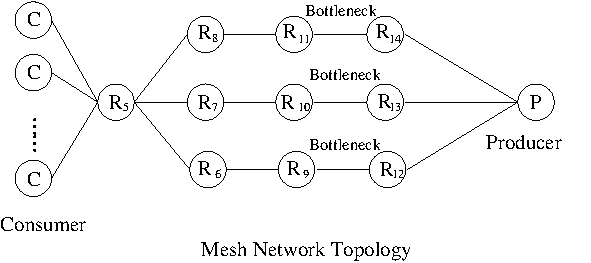
\includegraphics[width=2.5in]{mesh-topology.pdf}
	\caption{A mesh NDN network topology}
	\label{mesh-topology}
\end{figure}

In TCP/IP, only a single path is available for each source destination pair, and the forwarding process strictly follows the single path, thus adaptively selecting alternative path is very difficult. However, in NDN, the adaptive forwarding makes it possible. Taking the mesh network topology in Fig. \ref{mesh-topology} for example, a flow goes through $R5$. The flow has two available paths to get the data from provider. Router $R5$ can easily measure the congestion condition at the link1 (between router $R5$ and $R7$) and link2 (between router $R5$ and $R8$). If the router senses that link1 is much more congested than link2 then the router can adaptively forward the flow to link2. By such adaptive forwarding, the network resource can be effectively used and the flow complete time will be reduced.

However, such one-hop measurement is very limited. Taking the same situation for example, the true bottleneck happens on link3 (between router $R10$ and $R13$). But the router $R5$ can measure just one hop situation, it cannot sense the true bottleneck is on the link3, so it will still forward the Interest to link2. The wrong forwarding decision will put more burdens to link3, and increase the flow complete time of all the flows.

The SDN-style controller can get the whole network information. We will introduce the SDN's network-wide information to overcome the ``limited information'' problem. By the network-view information, the Interest can be forwarded to the best path. The whole network bandwidth utilization will be improved and total flow complete time can be reduced. So to improve the whole network bandwidth utilization and minimize total flow complete time, we further use SDN's network-wide information to design smart forwarding mechanism.

\subsection{ECN-based Interest sending rate}
We suppose every router fairly assigns its bandwidth to every flow. Our motivation is to send Interest at a maximum rate that the path can handle the corresponding coming back Data without dropping. To achieve this, every router on the path should calculates maximum Interest sending rate for the flows that goes through it. We define such rate of every router as $R_{r}$.

Fig.~\ref{fig-header} shows the Interest and Data ECN header. The ECN header contains the explicit congestion notification information on the path. The Interest carries the RTT(Round Trip Time) of the flow and this flow's Interest sending rate $R_{i}$. The RTT is defined as the interval between the time receiver sends an Interest to the time it receives the corresponding Data. In our design, RTT is used to determine the updating interval of $R_{r}$. The provider copies the Interest's RTT to Data when it send back the Data, and the routers do not change it along the path. As the first Interest of a flow does not know the RTT, we set the first Interest's RTT as 0. $R_{i}$ is the minimum $R_{r}$ of routers along flow $i$'s path. The router compares the $R_{i}$ that is recorded in the Data with its own $R_{r}$. If the router's rate is less than the one in the packet, it replaces it. By this way, the coming back Data carries the minimum $R_{r}$ of all the routers along the path. As the Data comes back along the same path of the Interest, the rate on the Data also reflects the path of the Interest. Each receiver sends its Interest according the $R_{i}$ it receives from Data.

\begin{figure}[t]
	\centering
	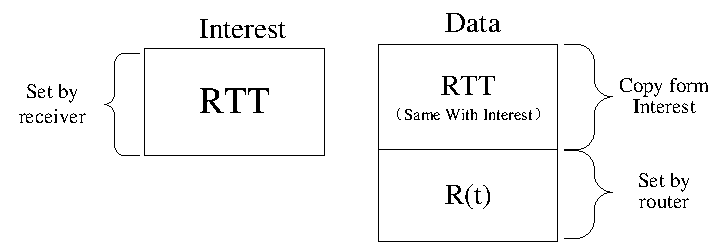
\includegraphics[width=2.5in]{header-ndn.pdf}
	\caption{Explicit congestion notification header for Interest and Data.}
	\label{fig-header}
\end{figure}

Suppose we know how many flows going through a link, then $R_{r}$ can be determined as follows:
\begin{equation}
	\label{eq:rt}
	R_{r}=\frac{C}{Flow_{num}*Size_{d}} \enspace .
\end{equation}
Where $Size_{d}$ is the size of incoming Data, $C$ is the bandwidth of the link, $Flow_{num}$ is the number of flows on the link. Eq.~\ref{eq:rt} is the ideal situation. When the network condition changes, such as a new flow is added, $R_{r}$ should be updated. To make the update process reasonable and let the system enter stable situation, Eq.~\ref{eq:rt} is improved as:
\begin{equation}
	\label{eq:updated_rt}
	R_{r}(t)=R_{r}(t-RTT_{avg})+\frac{\alpha(C-S(t))-\beta\frac{Q(t)}{RTT_{avg}}}{Flow_{num}*Size_{d}} \enspace
\end{equation}

Where $R_{r}(t)$ is the Interest sending rate that the router assigns to all flows at time $t$, $S(t)$ is the speed of coming back Data, $Q(t)$ is the packets in the queue at time $t$, $\alpha$ and $\beta$ are the parameters that influence the convergence and performance, $RTT_{avg}$ is the average RTT of all the flows that go through this router. We set $RTT_{avg}$ as the updating interval of $R_{r}(t)$. As Eq.~\ref{eq:updated_rt} shows, $\alpha$ influences how the bandwidth is used. If $\alpha$ is larger then bandwidth will be occupied quickly. Parameter $\beta$ influences how quickly that the packets in the queue can be drained. Obviously, larger $\alpha$ and $\beta$ can help the system to use the resource quickly. But larger $\alpha$ and $\beta$ will make the system become unstable, as the network is difficult to convergence. In Sec. \ref{sec:simulation}, we will further discuss the $\alpha$ and $\beta$'s influence to stability using evaluation results.

The definition of $R_{r}(t)$ in Eq.~\ref{eq:updated_rt} is explained as follows. The available bandwidth and queue should be fairly shared by all the flows, so the link's available resource is divided by the number of flow. If $(C-S(t))>0$, more available bandwidth could be used and the transmission rate of each flow should be increased. Otherwise, the bandwidth has been over used and the sending rate should be reduced. We assume that the packets in the queue should always come to zero. If it is not zero, it means too many Data packets flow into this link, and the Interest sending rate should be reduced. In every $RTT_{avg}$ the router should drain $Q(t)/RTT_{avg}$ Data packets. Because the $R_{r}(t)$ is the Interest sending rate, and the available resource is supplied to the Data, so we divide it by the size of Data.

If router tends to make the system converge to stable stage more quickly, it can update $R_{r}(t)$ with shorter interval $T$ $(0 < T \leq RTT_{avg})$. Then Eq.~\ref{eq:updated_rt} becomes:
\begin{equation}
	\label{eq:updated_rt3}
	R_{r}(t)=R_{r}(t-T)+\frac{\frac{T}{RTT_{avg}}\ast(\alpha(C-S(t))-\beta\frac{Q(t)}{RTT_{avg}})}{Flow_{num}*Size_{d}} \enspace .
\end{equation}
In NDN, Interests which have same prefix can be treated as in a same flow\cite{Flow}. And it is possible to calculate the number of flows that goes through a path by the prefix of Interest. However, using the prefix of the Interest name to estimate the number of flows traversing through the router will add complexity to the router. In\cite{RCP}, it has been proved that the processor-fair resource allocation method can estimate the flow number by the each flow's sending rate. Processor-fair means routers fairly allocate link bandwidth and queue resource to all flows through this link. Thus we also use process-fair resource allocation method to calculate the number of flows that go through this link:
\begin{equation}
	\label{eq:flownum}
	Flow_{num}=\frac{C}{R_{r}(t-RTT_{avg})\ast{Size_{d}}} \enspace .
\end{equation}

As we set every flow share the link bandwidth equally, and every flow's rate is the same, it is reasonable to use Eq.~\ref{eq:flownum} to estimate the number of flows. In Sec.~\ref{sec:simulation}, we will evaluate by simulation that the estimation is correctly.
Combining Eq.~\ref{eq:flownum} with Eq.~\ref{eq:updated_rt3} we have:
\begin{equation}
	\label{eq:updated_rt5}
	R_{r}(t)=R_{r}(t-T)[1+\frac{\frac{T}{RTT_{avg}}\ast(\alpha(C-S(t))-\beta\frac{Q(t)}{RTT_{avg}})}{C}] \enspace .
\end{equation}
Many factors may influence the size of Data in NDN, such as the different MTU of different link. So it will be very difficult to exactly measure the size of Data. When we need to use the size of Data to test the accuracy of the flow number estimation, we have to use the historical information to estimate the size of Data. From Eq.~\ref{eq:updated_rt5} we can find that, $R_{r}(t)$ does not need to measure the flow number directly and the size of Data. That greatly simplifies the router's calculating process.

\subsection{Smart adaptive forwarding}
In this paper we just control the forwarding process, not the route calculating process. In NDN, Data may have multiple replicas which are distributed in different hosts, so there are multiple paths to get a Data. And even the Data from the same provider may have different available paths. We assume the receivers have multiple paths to get a Data, and the routers have known every hop of different paths. The smart adaptive forwarding mechanism we proposed is independent from the route calculation.

We set that there is a controller to gather the network information. By the network information, the controller calculate the best forwarding decision and then inform the routers. Every router sends its own $R_{r}(t)$, the transmit delay and the bandwidth of the next hop to the controller at an interval of $RTT_{avg}$. After several $RTT_{avg}$, the controller can know every router's $R_{r}(t)$ and the transmit delay of every hop. We denote the information as forwarding-assistant information. The network's route information can also be stored in the controller. The forwarding-assistant and route information stored in the controller is showed in Fig.~\ref{fig-assistant-information}. As Fig.~\ref{fig-assistant-information} shows, the forwarding-assistant information table contains the $R_{r}(t)$, the transmit delay and the bandwidth of every router in the network. The route information record that through what paths Interest can get its Data. For example, Interest with prefix1 can get its corresponding Data from two path: R1-R2-R3 and R1-R4-R3. By the forwarding-assistant information and route information, we can calculate the best forwarding strategy.

\begin{figure}[t]
	\centering
	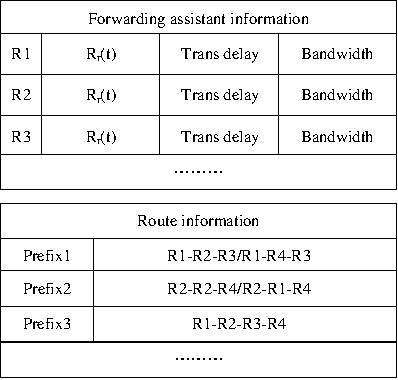
\includegraphics[width=2.5in]{forwarding-assistant-information.pdf}
	\caption{Forwarding assistant and route information stored in the controller.}
	\label{fig-assistant-information}
\end{figure}

Using the Interest sending rate we propose above, the FCT of each flow is:
\begin{equation}
	\label{eq:fct}
	FCT=\frac{Size_{f}}{Size_{d}\ast{R_{b}}}+RTT
\end{equation}
where $Size_{f}$ is the size of the flow, $R_{b}$ is the bottleneck router's Interest sending rate. Eq.~\ref{eq:fct} means that FCT is the time that the flow goes through the bottleneck plus the RTT of this flow. The RTT of this flow can be calculated by the forwarding-assistant information.

We suppose the $i$-th flow has several available paths. If it chooses path $j$, then this flow's FCT on path $j$ should be:
\begin{equation}
	\label{eq:fctij}
	FCT_{i,j}=\frac{Size_{f}}{Size_{d}\ast{R^{'}_{b}}}+RTT_j
\end{equation}
where $RTT_j$ is the RTT of flow $i$ if it chooses path $j$ and $R^{'}_{b}$ is the bottleneck router's Interest sending rate on path $j$.

\begin{equation}
R^{'}_{b}=\frac{C}{Flow_{num}+1} = \frac{C}{C/(R_{b}\ast{Size_{d}})+1}
\end{equation}
For simplicity, we set the value of $Size_{d}$ and $Size_{f}$ as fixed values, and suppose $Size_{data} =Size_{flow}$. So Eq.~\ref{eq:fctij} becomes:
\begin{equation}
FCT_{i,j}=\frac{C/(R_{b}*Size_{d})+1}{C}+RTT_j
\end{equation}

Our design goal is to minimize the Total Flow Complete Time (TFCT) in the network. TFCT is the sum of all the flows' complete time. To achieve our goal we define the objective of the smart forwarding as:
\begin{equation}
	\begin{aligned}
		& \min &&  \sum_{i=0}^{n} FCT_i \\
		& \text{s.t.}  && \text{path } j \text{ is available};\\
		&              && \forall i, P_i \in \{0,1\};\\
		&              && \max \min  R_i \enspace .
	\end{aligned}
\end{equation}
Where $P_i$ is the number of paths that flow $i$ chooses, $R_i$ is flow $i$'s Interest sending rate. $P_i \in \{0,1\}$ means flow $i$ can choose at most one path. $max min \ R_i$ means flow $i$'s Interest sending rate should be maximized. The reason we maximize $R_i$ is to achieve fairness between different flows. If we do not set $max min \ R_i$, some flows may choose a min $R_i$ to minimum the TFCT, and that will influence this flow's FCT.
% Sacrificing oneself to achieve the goal of minimum TFCT is unfair.

Routers send the updated forwarding-assistance and route information to the controller at the interval of $RTT_{avg}$. The controller sends back smart forwarding decision for each flow when it receives the router's updating information. The smart forwarding decision is based on the unit of flow, not the unit of packet. So the overhead introduced by the controller's help is limited compared with the whole volume that goes through the router. To timely reflect the change of network information to the controller, routers can change the sending interval, and that will raise the overhead. The balance between the overhead and the accuracy of updating information can be adaptively controlled.

